\section{Régression polynomiale}

Nous avons précédemment démontré à plusieurs reprises que notre système comporte un nombre insuffisant de caractéristiques, notre bias est élevé \textit{(sous-apprentissage)}. \\
À l'aide de la fonction \ref{lst:polyFeatures} nous pouvons augmenter le nombre d'entités de $X$, c'est-à-dire les données du niveau de l'eau. L'objectif est de réaliser un nouveau vecteur contenant $X$ allant de la puissance~1 à $p$, chaque colonne représente une 
puissance différente. 

\begin{figure}[!h]
\begin{minted}[frame=lines, framesep=2mm, baselinestretch=1.2, fontsize=\footnotesize, linenos, breaklines=true]{python}
def polyFeatures(X, p):
    X_poly = np.zeros((X.shape[0], p))
    for i in range(1,p+1):
        X_poly[:,i-1] = X[:,0]**i
    return X_poly
\end{minted}   
\captionof{listing}{\label{lst:polyFeatures}Fonction polyFeatures}
\end{figure}


\subsection{Apprentissage de la régression polynomiale}

Finalement, nos données deviennent des termes polynomiaux. Dans ce cas, le principe de régression est le même, nous avons simplement augmenté le nombre de caractéristiques pour 
éviter le sous-apprentissage. 
Cependant, élever à la puissance nos termes peut donner des valeurs différentes et non régulières, nous allons donc normaliser nos données avant de réaliser la régression linéaire et afficher nos courbes d'apprentissage.

\begin{figure}[!h]
    \begin{minipage}{.48\linewidth}
        \begin{center}
            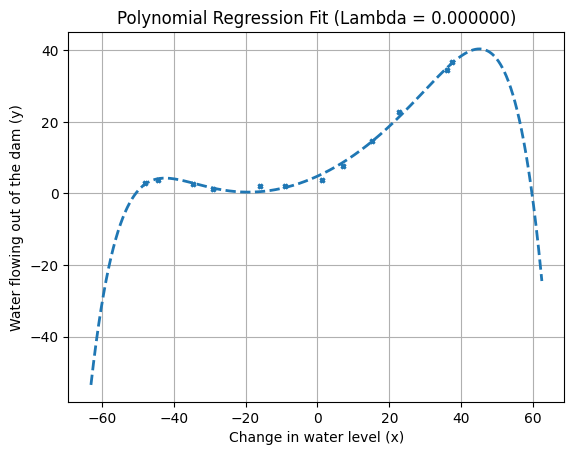
\includegraphics[width=.8\textwidth]{./img/5.1(1).png}
            \caption{\label{fig:reg-poly-0}Régression polynomiale $\lambda = 0$}  
        \end{center}
    \end{minipage}\hfill
    \begin{minipage}{.48\linewidth}
        \begin{center}
            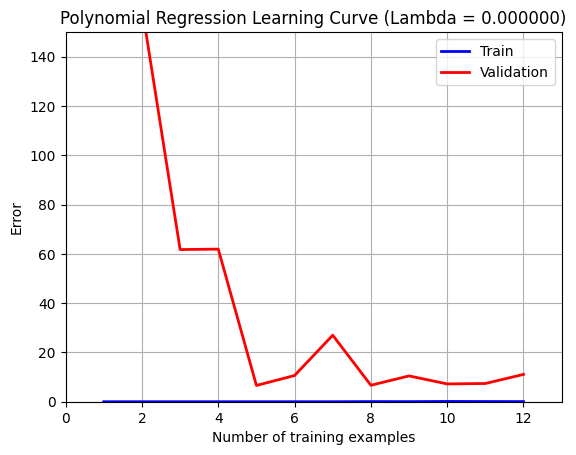
\includegraphics[width=.8\textwidth]{./img/5.1(2).png}
            \caption{\label{fig:learning-curve-poly-0}Courbe d'apprentissage $\lambda = 0$}  
        \end{center}
    \end{minipage}
\end{figure}

Dans ce premier cas, nous n'avons pas appliqué de régulation, comme pour la partie~1, $\lambda = 0$. \\
Avec un thêta de dimension~2, nous avions constaté un sous-apprentissage, ici c'est l'inverse. On le constate dans un premier temps avec la figure \ref{fig:reg-poly-0}, où notre régression linéaire est particulièrement ajustée à notre ensemble de données. Par la suite la figure 
\ref{fig:learning-curve-poly-0}, nous montre que notre erreur d'entrainement est très faible. La présence d'une variance élevée entre l'erreur d'entrainement et de validation nous suggère que nous sommes en surapprentissage.

\subsection{Réglage du paramètre de régularisation $\lambda$}\label{sec:select-lambda}

Maintenant que nous sommes en surapprentissage avec $\lambda = 0$, nous allons utiliser notre régulation mise en œuvre dans la partie~1 pour différentes valeurs grâce au code suivant.


\begin{figure}[!h]
\begin{minted}[frame=lines, framesep=2mm, baselinestretch=1.2, fontsize=\footnotesize, linenos, breaklines=true]{python}
for Lambda in [0, 1, 100]:
    theta = trainLinearReg(X_poly, y, Lambda, maxiter=10)
    error_train, error_val = learningCurve(X_poly, y, X_poly_val, yval, Lambda)
    # Plot training data and fit & learning curves (Error vs Number of training examples)
    # code donné...
\end{minted}   
\captionof{listing}{\label{lst:plot-lambda-test}Régularisation pour différent $\lambda$}
\end{figure}
    


\begin{figure}[!h]
    \begin{minipage}{.48\linewidth}
        \begin{center}
            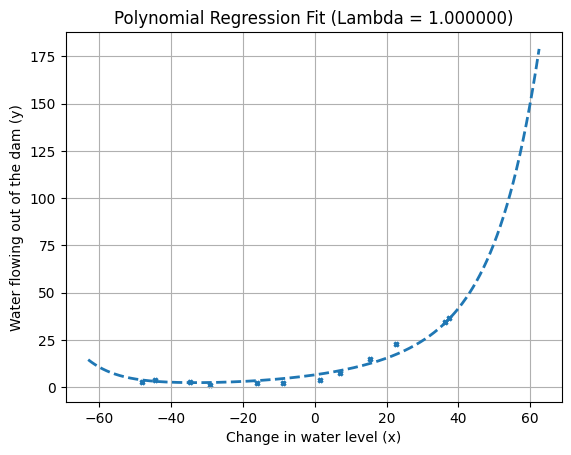
\includegraphics[width=.8\textwidth]{./img/5.2(1).png}
            \caption{\label{fig:reg-poly-1}Régression polynomiale $\lambda = 1$}  
        \end{center}
    \end{minipage}\hfill
    \begin{minipage}{.48\linewidth}
        \begin{center}
            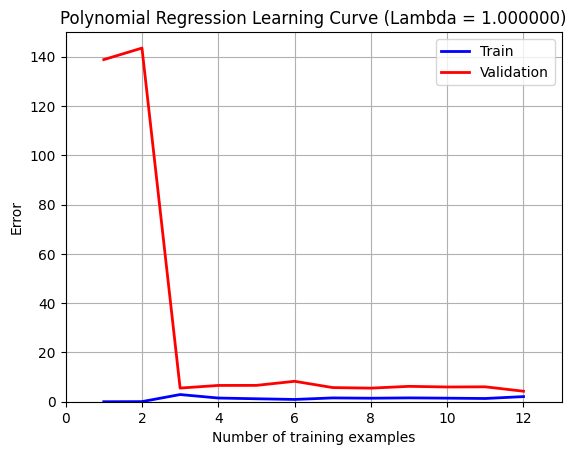
\includegraphics[width=.8\textwidth]{./img/5.2(2).png}
            \caption{\label{fig:learning-curve-poly-1}Courbe d'apprentissage $\lambda = 1$}  
        \end{center}
    \end{minipage}
\end{figure}


\begin{figure}[!h]
    \begin{minipage}{.48\linewidth}
        \begin{center}
            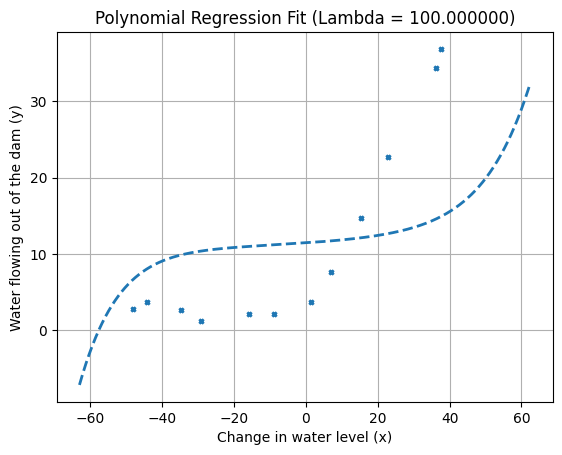
\includegraphics[width=.8\textwidth]{./img/5.2(3).png}
            \caption{\label{fig:reg-poly-100}Régression polynomiale $\lambda = 100$}  
        \end{center}
    \end{minipage}\hfill
    \begin{minipage}{.48\linewidth}
        \begin{center}
            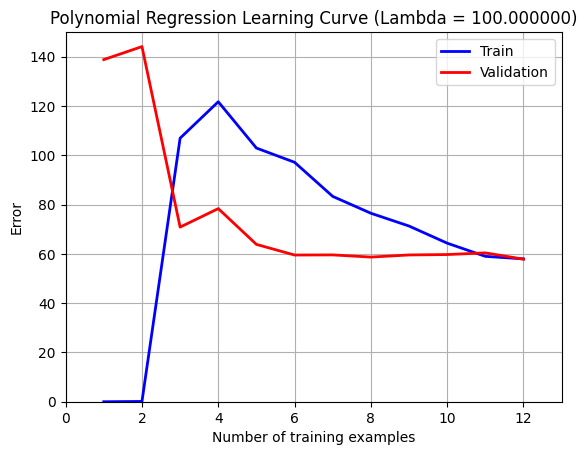
\includegraphics[width=.845\textwidth]{./img/5.2(4).png}
            \caption{\label{fig:learning-curve-poly-100}Courbe d'apprentissage $\lambda = 100$}  
        \end{center}
    \end{minipage}
\end{figure}

Pour $\lambda = 1$, nos résultats sont satisfaisants. L'erreur d'apprentissage est faible ainsi que l'erreur de validation. Alors que pour $\lambda = 100$, nous pouvons observer une erreur importante et donc un bias élevé \textit{(sous-apprentissage)}.
Nous pouvons considérer que la valeur de $\lambda$ la plus appropriée est proche de 1.

\subsection{Sélection de $\lambda$ avec un jeu de validation}


Nous avons pu constater qu'une valeur appropriée pour $\lambda$ se rapproche de 1, mais il ne serait pas judicieux d'affiner notre paramètre manuellement. Pour ce faire nous allons entrainer notre modèle pour une différente valeur de $\lambda$ puis calculer nos erreurs. Il est 
important à noter que pour calculer nos erreurs nous pouvons utiliser notre fonction \textit{linearRegCostFunction} avec une valeur de $\lambda = 0$.

\vspace{.2cm}

\begin{figure}[!h]
\begin{minted}[frame=lines, framesep=2mm, baselinestretch=1.2, fontsize=\footnotesize, linenos, breaklines=true]{python}
def validationCurve(X, y, Xval, yval):
    lambda_vec = np.array([0, 0.001, 0.003, 0.01, 0.03, 0.1, 0.3, 1, 3, 10])
    error_train = np.zeros(lambda_vec.size)
    error_val = np.zeros(lambda_vec.size)

    for index, Lambda in enumerate(lambda_vec):
        theta = trainLinearReg(X, y, Lambda)
        error_train[index], _ = linearRegCostFunction(X, y, theta, 0)
        error_val[index], _ = linearRegCostFunction(Xval, yval, theta, 0)

    return lambda_vec, error_train, error_val

""" output
 Lambda    Train Error  Validation Error
 0.000000   0.052931    11.079058
 0.001000   0.137758    12.755159
 0.003000   0.172035    16.593054
 0.010000   0.221503    16.946651
 0.030000   0.281857    12.831260
 0.100000   0.459305    7.587272
 0.300000   0.921748    4.636853
 1.000000   2.076202    4.260622
 3.000000   4.901350    3.822897
 10.000000  16.092208   9.945501
"""
\end{minted}   
\captionof{listing}{\label{lst:validationCurve}Fonction validationCurve}
\end{figure}

\vspace{.2cm}

\begin{figure}[!h]
    \begin{minipage}{.44\linewidth}
        Après avoir tracé nos erreurs en fonction de $\lambda$, nous pouvons sélectionner une valeur $\lambda$ pour laquelle notre erreur de validation est minimale. \\
        La courbe de validation nous indique que l'erreur est minimale pour une valeur de $\lambda \approx 3$. Si l’on analyse plus en détail la sortie de notre fonction validationCurve, on constate que pour $\lambda = 3$ notre erreur de validation est 
        de 3.822897. \\

        Pour la suite de ce TP nous choisirons donc $\lambda = 3$ comme paramètre de régularisation.
    \end{minipage}\hfill
    \begin{minipage}{.56\linewidth}
        \begin{center}
            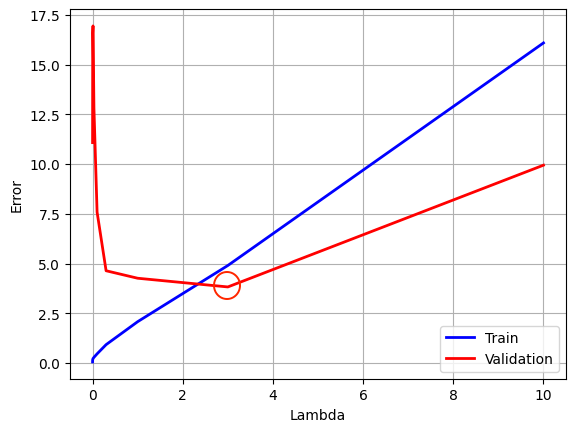
\includegraphics[width=.9\textwidth]{./img/5.3.png}
            \caption{\label{fig:validation-curve-poly}Courbe de validation en fonction de $\lambda$}  
        \end{center}
    \end{minipage}
\end{figure}


\subsection{Calcul de $J_{test}(\theta)$}

Nous savons que notre modèle est efficace pour des données qu'il connait, c'est-à-dire celles que nous avons utilisées pour entrainer notre modèle. Quand est-il pour un ensemble de données inconnus, \textit{Xtest} ou \textit{X\_poly\_test} sous forme polynomiale\,? 
Pour entrainer notre modèle, nous avons sélectionné les paramètres précédents, considérés comme optimaux: \textit{X\_poly, y, Lambda=3, maxiter=100}.

\begin{figure}[!h]
\begin{minted}[frame=lines, framesep=2mm, baselinestretch=1.2, fontsize=\footnotesize, linenos, breaklines=true]{python}
Lambda = 3
theta = trainLinearReg(X_poly, y, Lambda, maxiter=100)

Jtest, _ = linearRegCostFunction(X_poly_test, ytest, theta, 0) # Lambda=0, pas de régularisation pour déterminer l'erreur
print("The test set error is:", Jtest)

"""output
The test set error is: [3.85989019]
"""
\end{minted}   
\captionof{listing}{\label{lst:validationCurve}Fonction validationCurve}
\end{figure}

L'erreur obtenue pour notre ensemble de données inconnues par le modèle est de 3.85989019, ce qui est plus que satisfaisant, notre résultat est proche de l'erreur obtenue pour un jeu de donnée connue. Nous pouvons considérer que notre modèle est correctement 
paramétré.

\vspace{.5cm}
    
\subsection{Exerice facultatif}

\begin{figure}[!h]
    \begin{minipage}{.44\linewidth}
        Dans le cas de petit ensemble d'apprentissages comme le nôtre, il est parfois plus intéressant de tracer nos courbes sur la moyenne des erreurs de plusieurs exemples choisis au hasard. \\

        Dans notre cas nous avons un ensemble de longueurs~12, l'idée serait donc de choisir au hasard un certain nombre d'échantillons de cet ensemble, d'obtenir les thêta minimaux et de calculer les erreurs d'entrainement et de validation.\\
        Il faut réaliser c'est étapes un certain nombre de fois, puis faire la moyenne de nos erreurs. L'algorithme est assez simple \textit{(cf bloc de code \ref{lst:random-sample})}. \\


    \end{minipage}\hfill
    \begin{minipage}{.56\linewidth}
        \begin{center}
            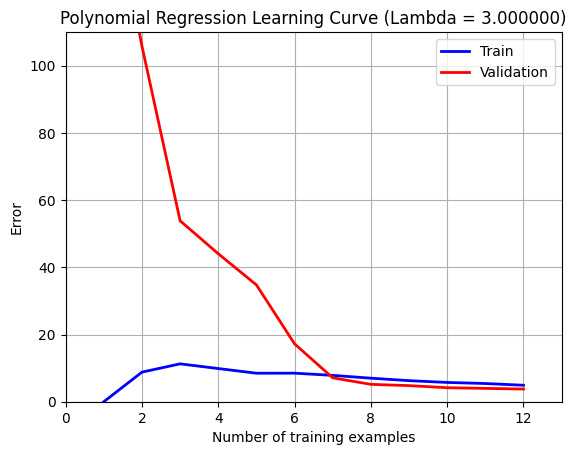
\includegraphics[width=.9\textwidth]{./img/5.5.png}
            \caption{\label{fig:validation-curve-poly}Courbe de validation en fonction de $\lambda$}  
        \end{center}
    \end{minipage}
\end{figure}

Après avoir obtenu la moyenne de nos erreurs, nous pouvons tracer l'erreur d'entrainement et de validation en fonction du nombre d'échantillons. Dans notre cas, nous avons sélectionné une valeur de $\lambda = 3$, pour comparer les résultats avec ceux précédemment obtenus. \\
Nous pouvons considérer à l'aide de la figure \ref{fig:validation-curve-poly} que notre modèle est bien entrainé, nous n'observons pas de variance ou de bias élevé. L'erreur obtenue est proche des résultats précédents.



\begin{figure}[!h]
\begin{minted}[frame=lines, framesep=2mm, baselinestretch=1.2, fontsize=\footnotesize, linenos, breaklines=true]{python}
num_iterations = 50
Lambda = 0.01
errors_train = []
errors_val = []

i = np.random.randint(5, len(X) + 1) # sélection de i hasardeuse

for _ in range(num_iterations):
    i_train = np.random.choice(len(X), i, replace=False) # sélection des échantillons dans X
    i_val = np.random.choice(len(Xval), i, replace=False) # sélection des échantillons dans Xval
    
    X_random = X_poly[i_train]  
    y_random = y[i_train]
    X_val_random = X_poly_val[i_val] 
    y_val_random = yval[i_val]

    X_random = np.column_stack((np.ones(X_random.shape[0]), X_random)) # ajout du terme bias
    X_val_random = np.column_stack((np.ones(X_val_random.shape[0]), X_val_random))
        
    theta = trainLinearReg(X_random, y_random, Lambda, maxiter=100) # entrainement du modèle
    error_train, error_val = learningCurve(X_random, y_random, X_val_random, y_val_random, Lambda) # calcul des erreurs

    errors_train.append(error_train) # sauvegarde des erreurs
    errors_val.append(error_val)
    
error_train = np.mean(np.array(errors_train), axis=0) # moyenne des erreurs
error_val = np.mean(np.array(errors_val), axis=0)

plt.figure()  # plot des erreurs en fonction du nombre d'échantillons 
plt.plot(range(1,i+1), error_train, color='b', lw=2, label='Train')
plt.plot(range(1,i+1), error_val, color='r', lw=2, label='Validation')
plt.title('Polynomial Regression Learning Curve (Lambda = %f)' % Lambda)
plt.xlabel('Number of training examples')
plt.ylabel('Error')
plt.xlim(0, i+1)
plt.ylim(0, 110)
plt.legend()
plt.grid()
\end{minted}   
\captionof{listing}{\label{lst:random-sample}Calcul des erreurs avec plusieurs échantillons choisis au hasard}
\end{figure}


